\chapter{Background}
\label{ch:background_report}

This chapter discusses the key concepts that are required to understand the thesis work.

\section{Static Analysis}

In the last few years, we see the enormous increase in the usage of software. We see software everywhere in the walk of our life with the Internet of Things, for example. As the usage increases, it stresses quality as being more secure and does not break. Earlier, software developers used to do manual auditing of the code, but sooner they realised it is time consuming and so planned to automate the process. Therefore, different testing mechanisms evolved, such as black-box testing, white-box testing. \\

Static analysis falls under the category White-box testing. It tests the software without executing the code, and therefore the name means it. On the other side, tools are testing with a mechanism by executing the code, which is called dynamic testing. We also call static analysis as ‘Source Code Analysis’. The uses of static analysis tools are such as compiler optimisation, coding support and detection of security vulnerabilities and bugs. \cite{deca} It reports bugs such as injections, cross-site scripting (XSS), buffer overflow, and dead code. \cite{bugs} There are different techniques followed for analysing source code. One example as ‘Data Flow Analysis’, it tests the source code by dividing into basic blocks. \cite{Woegerer} Here is an example; a php program, as seen below, is divided into blocks, and they consider each block as one node.

\begin{lstlisting}[showstringspaces=false, language=PHP][frame=single]

$a = 0;
$b = 1;

if ($a == $b)
{ # start of block
echo "a and b are the same";
} # end of block
else
{ # start of block
echo "a and b are different";
} # end of block


\end{lstlisting}

After that, a path is formed by connecting the nodes along the control flow, as seen in the  \autoref{fig:CFG}. \\

\begin{figure}
	\centering
	
	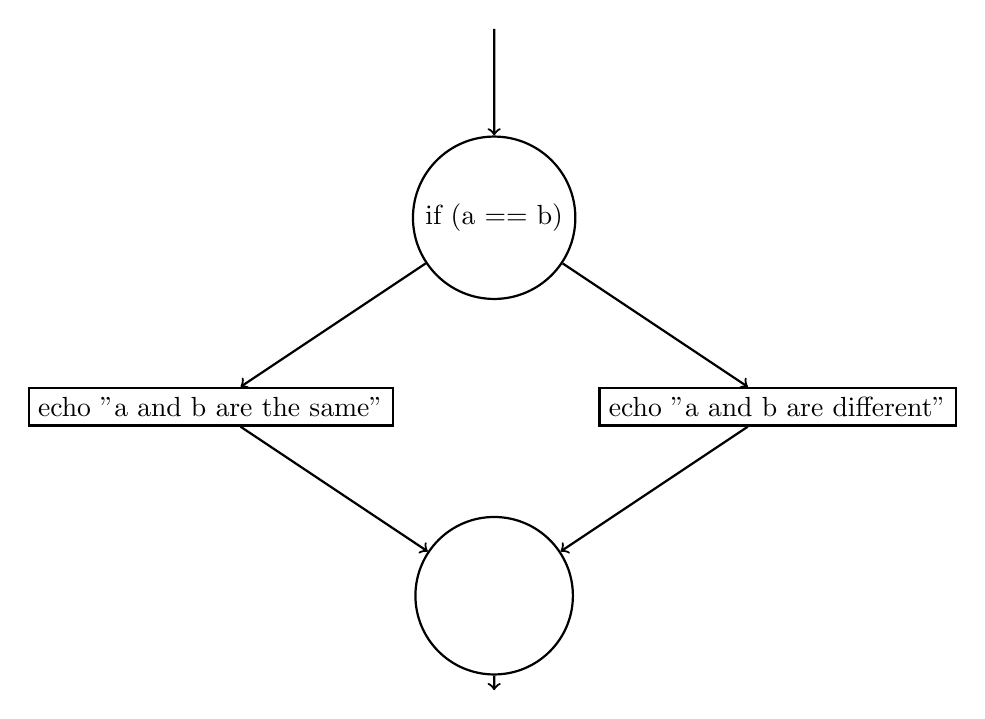
\begin{tikzpicture}[thick,scale=0.6, every node/.style={scale=0.6}]
	
	\begin{scope}[every node/.style={circle,thick,draw}]
	\node (node 1) at (4,8) {if (a == b)};
	\node[rectangle] (node 2) at (-2,4) {echo "a and b are the same"};
	\node[rectangle] (node 3) at (10,4) {echo "a and b are different"};
	\node[circle,minimum size=2cm] (node 4) at (4,0) {}; 
	\end{scope}
	
	\begin{scope}
	\draw [->] (4,12) -- (node 1);
	\path [->] (node 1) edge node[right] {} (node 2);
	\path [->] (node 2) edge node[right] {} (node 4);
	\path [->] (node 1) edge node[right] {} (node 3);
	\path [->] (node 3) edge node[right] {} (node 4);
	\draw [->] (node 4) -- (4,-2);
	
	\end{scope}
	
	\end{tikzpicture} 
	
	\caption{Control Flow Graph}
	\label{fig:CFG}
\end{figure} 


There are different kinds of tools available for doing static code analysis such as IDE notifications, IDE tools, dedicated tools, Linters and CLI tools. Out of which, the dedicated tools and CLI tools are more likely to report security vulnerabilities, whereas others are more likely to report coding style issues. In this thesis, we will look into the usability aspect of such tools.


\section{Usability}

The Human-Computer Interaction researcher, Dr Jakob Nielsen, defines usability as “a quality attribute that assesses how easy user interfaces are to use”. \cite{usability-define} They characterise it by five quality elements:

\begin{enumerate}
\item \textbf{Learnability:} It says whether the design is simple for the person seeing the design for the first time, and he can understand it.
\item \textbf{Efficiency:} After getting familiar with design, how simple is it to do the tasks in a shorter time as possible?
\item \textbf{Memorability:} Once the person knew the design and worked for some time and later when he comes back after some significant time, then is the design helpful enough to memorise?
\item \textbf{Errors:} It signifies the possibility of a person encountering the design make some errors and then whether he could recover from it quickly.
\item \textbf{Satisfaction:} It determines the delightfulness of the person using the design.
\end{enumerate}

\section{Wireframe}

A wireframe is a methodology of showing a blueprint for a particular product. For example, if we consider wireframing a user interface of an application. It means to show a blueprint design of how the application UI look like with different elements such as buttons, text boxes placed on it and also how they interact and navigate to other User Interfaces. The blueprint design could vary from low fidelity, i.e., rough sketches to high fidelity, i.e., a closer look to the desired final UI. There are several tools available in the market to wireframe and Balsamiq \cite{B} is one such tool. It is a prototyping the actual product with a precise simulation in functionality and visualisation of the actual product to some extent. The advantage of this is the easiness of finding the mistakes in design earlier and so the cost of fixing them would be less. Here is an example of a wireframe done to a website idea. It is about how it should look and the elements we would like to see as on an end product, i.e., final front-end design of the website coded. It is shown in the following \autoref{fig:wireframe_website} of what one could design using Balsamiq tool and discuss with peers how they feel or to oneself to draw the ideas of what they want to attain before coding to get the web page with the desired UI. \\ \\


\begin{figure}[hbt!]
	\centering
	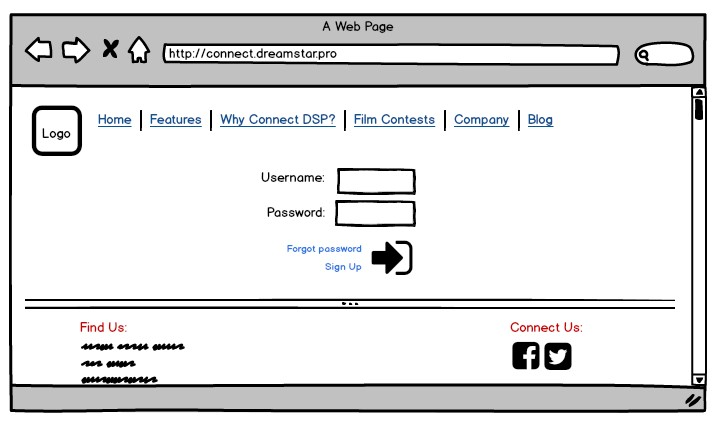
\includegraphics[width=\linewidth]{figures/Connect_DSP}
	\caption{An Example to Wireframe a Website.\cite{B}}
	\label{fig:wireframe_website}
\end{figure}

\let\cleardoublepage\clearpage